\documentclass[a4paper,11pt]{report}

\usepackage{fullpage}

\usepackage{amsmath}
\usepackage{bussproofs}
\usepackage{mathpartir}
\usepackage{prooftrees}
\usepackage{color}

% Minted
\usepackage[cache=false]{minted}

\newmintinline{c}{
  fontsize=\small,
  breaklines=true
}

\newminted{c}{
  frame=single,
  framesep=2mm,
  fontsize=\scriptsize,
  mathescape
}

\newminted[clinecode]{c}{
  frame=single,
  framesep=2mm,
  fontsize=\scriptsize,
  mathescape,
  linenos
}

\newcommand*{\BBox}[1]{\draw (#1 + 0.5,0.5) -- (#1 + 1.5,0.5) -- (#1 + 1.5,-0.2)
  -- (#1 + 0.5,-0.2) -- cycle;}
\newcommand*{\SBox}[1]{}

\newcommand*{\equal}{=}

% for finite state automata
\usepackage{tikz}
\usetikzlibrary{automata,positioning}

\author{Sylvain Julmy}
\date{\today}

\setlength{\parindent}{0pt}

\begin{document}

\begin{center}
  \Large{
    System-oriented Programming\\
    Spring 2018
  }
  
  \noindent\makebox[\linewidth]{\rule{\linewidth}{0.4pt}}
  S03
  \noindent\makebox[\linewidth]{\rule{\linewidth}{0.4pt}}

  \begin{flushleft}
    Professor : Philippe Cudré-Mauroux

    Assistant : Michael Luggen
  \end{flushleft}
  
  \noindent\makebox[\linewidth]{\rule{\linewidth}{0.4pt}}

  Submitted by Sylvain Julmy
  
  \noindent\makebox[\linewidth]{\rule{\textwidth}{1pt}}
\end{center}

Note : the complete source file are available inside the zipped file.

\section*{Exercice 1}

\subsection*{a)}

\begin{ccode}
for (low = 0; low <= high; low++)
        printf("%i\n", low);
\end{ccode}

\subsection*{b)}

\begin{ccode}
if (low > high) goto end;
do
{
    printf("%i\n", low);
    low++;
} while (low <= high);

end:
\end{ccode}

We use a $goto$ and an $if$ in order to don't go inside the loop if $low > high$.

\section*{Exercice 2}

\subsection*{a)}

\begin{ccode}
i = 0;
start:
printf("%i\n",i++);
if (i < n) goto start;
\end{ccode}

\subsection*{b)}

\begin{ccode}
if (i == 1) goto case1;
if (i == 2) goto case2;
goto caseDefault;

case1 :
printf("case 1 \n");
goto end; // break

case2 :
printf("case 2 \n");

caseDefault:
printf("default case \n");
goto end; // unnecessary, but we follow the code example

end:;
\end{ccode}

\subsection*{c)}

\begin{ccode}
for (i = 0; i < n; i++)
{
    printf("action 1, i=%i\n", i);
    if (i > 0) goto end;
    printf("action 2, i=%i\n", i);
}
end:;
\end{ccode}

\subsection*{d)}

\begin{ccode}
for (i = 0; i < n; i++)
{
    printf("action 1, i=%i\n", i);
    if (i > 0) goto loopEnd;
    printf("action 2, i=%i\n", i);
    loopEnd:;
}
\end{ccode}

Note : we have to put a semi-colon after the label declaration if there is no
following instructions, $;$ alone acts for the $nop$ instruction.

\newpage

\section*{Exercice 3}

Figure~\ref{fig:gdb-script} show the list of command to execute, as well as some
comment, in order to detect the causes of the crash.

\begin{figure}[ht]
  \centering
\begin{verbatim}
// run first time to show the error
run
// set breakpoint and add display for both expr i and N
break 16
display i
display N
// rerun and answer yes when asking for reruning the program
run
// stop each time on the breakpoint
c     c     c
// now we clearly see that N/i is 3/0 and would lead to a arithmetic error
c
// and now the following message is display :
Program received signal SIGFPE, Arithmetic exception.
0x00005555555546d0 in main () at ex3/div_zero.c:12
\end{verbatim}
  \caption{\label{fig:gdb-script} List of gdb command to execute in order to
    clearly show the error from program \ref{lst:div-zero}.}
\end{figure}

\begin{listing}[ht]
\centering
\begin{clinecode}
#include <stdio.h>

int N = 3;

int main()
{
   int ctr, i;
   int res;

   i = N;
   res = N;

   printf("res  N  i\n");
   for (ctr = 0; ctr <= N; ++ctr, --i)
   { // 'ctr <= N' for exercice 5
      res = N / i;
      printf("%3i%3i%3i\n", res, N, i);
   }

   return 0;
}
\end{clinecode}
\caption{C program that would have an arithmetic error, a division by zero.}
\label{lst:div-zero}
\end{listing}

\newpage

\section*{Exercice 4}

Figure~\ref{fig:gdb-script-b} show the list of command to execute, as well as some
comment, in order to detect the causes of the crash.

\begin{figure}[ht]
  \centering
\begin{verbatim}
// First we create a core file using the generate-core-file command from gdb
// then we load it with (filename of the core file is core.17331)
gdb div_zero core.17331 --tui

// then we can directly watch the varible and saw why the program crashed
display N
display i

// we saw N = 3 and i = 0, then N/i is an arithmetic error :

Core was generated by `/home/snipy/Master/mcs-git/sys-oriented-prog
                       /exercices/s03/exercices/div_zero'.
Program terminated with signal SIGFPE, Arithmetic exception.
#0  0x00005555555546d0 in main () at ex3/div_zero.c:16
(gdb) display N
1: N = 3
(gdb) display i
2: i = 0
(gdb) 
\end{verbatim}
  \caption{\label{fig:gdb-script-b} List of gdb command to execute in order to
    clearly show the error from program \ref{lst:div-zero} with the line 16
    modified.}
\end{figure}

\section*{Exercice 5}

\begin{ccode}
n=2*m+n;
\end{ccode}

Abstract Syntax Tree :

\begin{forest}
  [$n \equal 2*m+n$
  [$\equal$
  [$\&n$]
  [$+$
  [$*$
  [$2$]
  [$m$]
  ]
  [$n$]
  ]
  ]]
\end{forest}

Control Stack :

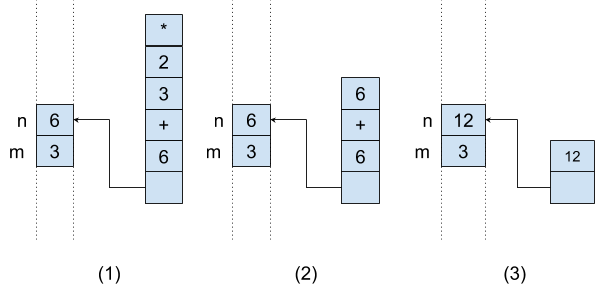
\includegraphics[width=0.7\textwidth]{figures/5a}

\begin{ccode}
n*=m+1
\end{ccode}

Abstract Syntax Tree :

\begin{forest}
  [$n *\equal m + 1$
  [$\equal$
  [$\&n$]
  [$*$
  [$n$]
  [$+$
  [$m$] [$1$]
  ]
  ]
  ]
  ]
\end{forest}

Control Stack :

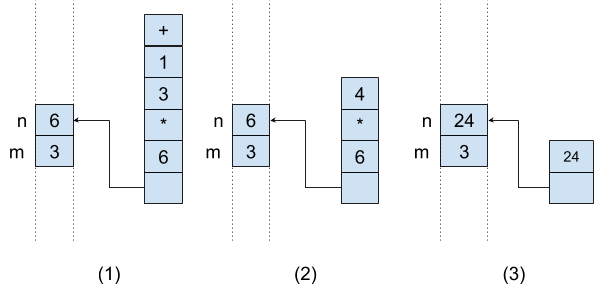
\includegraphics[width=0.7\textwidth]{figures/5b}

\end{document}
